%---------------------------------------------------------------------------------
%--------------------------Set the variables for every client---------------------
%---------------------------------------------------------------------------------
\renewcommand{\hostname}{DeepThought}
\renewcommand{\os}{Earth}
\renewcommand{\ip}{42.42.42.23}
\renewcommand{\tcpports}{1,2,3}
\renewcommand{\udpports}{23,42}
\renewcommand{\vuln}{Vogons}
%%%Did you get root? Comment out if you only got low priv access
\def\root{}   %%% Define root if you got root shell

%----------------------------------------------------------------------------------
%-------------------------------Auto generated content-----------------------------
%----------------------------------------------------------------------------------

\section{\hostname}
\subsection{Service Enumeration}

\begin{table}[h]
	\begin{tabular}{|c|c|}
		\hline
		\multicolumn{2}{|c|}{\textbf{\hostname}}\\\hline\hline
		Type         & Open ports   \\\hline
		TCP          & \tcpports{}  \\\hline
		UDP          & \udpports{}  \\\hline\hline
		\textbf{\os} & \textbf{\ip} \\\hline
	\end{tabular}
	\caption{Service enumeration \hostname}
\end{table}

\subsection{Remote Access Exploitation}

\paragraph{Vulnerability Exploited:}
\vuln

%----------------------------------------------------------------------------------
%-------------------------------Start writing here---------------------------------
%----------------------------------------------------------------------------------

\paragraph{Vulnerability Explanation:}
BLA BLA WRITE SOMETHING HERE 



\paragraph{Severity:}
\textbf{\textcolor{red}{Critical}}

\paragraph{Proof of Concept:} 
\begin{lstlisting}[caption={Exploitation of \hostname}]
*@Kali prep:@*

*@Modifications in the exploit@*
PANIC **@PANIC@** PANIC
*@Running the exploit@*

*@Escaping the low priv shell:@*
\end{lstlisting}


\begin{figure}[H]
\centering
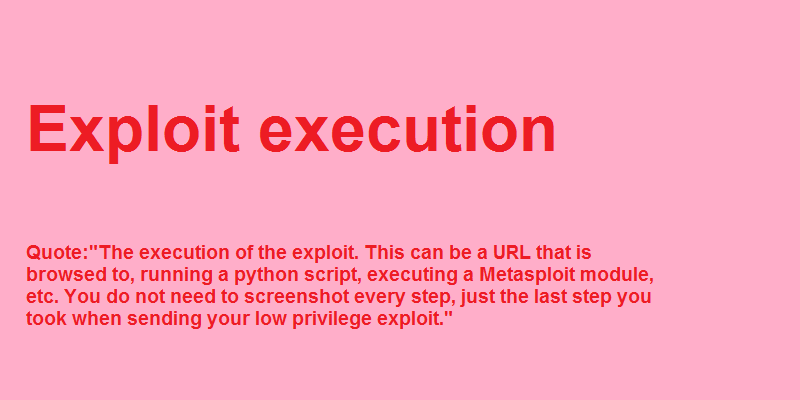
\includegraphics [width=\textwidth]{./hosts/\hostname/exploitexecution.png}
%scale 0.5 bedeutet 50% der originalgröße
%angle=90 Grafik um 90° drehen
\caption[Exploitation of \hostname]{Exploitation of \hostname} \label{\hostname-1}
\end{figure}


\ifdefined\root
   

%Conditional Privilege Escalation Block .. --------------------------------------------------------------------------------------------------------------------


%Part for Priv escalation -------------------------------------------------------------------------------------------
\subsubsection{Privilege Escalation}




\begin{figure}[H]
\centering

\includegraphics [width=\textwidth]{./hosts/\hostname/local.png}
%scale 0.5 bedeutet 50% der originalgröße
%angle=90 Grafik um 90° drehen
\caption[Local shell of \hostname]{Local shell of \hostname} \label{\hostname-2}
\end{figure}


\begin{figure}[H]
\centering
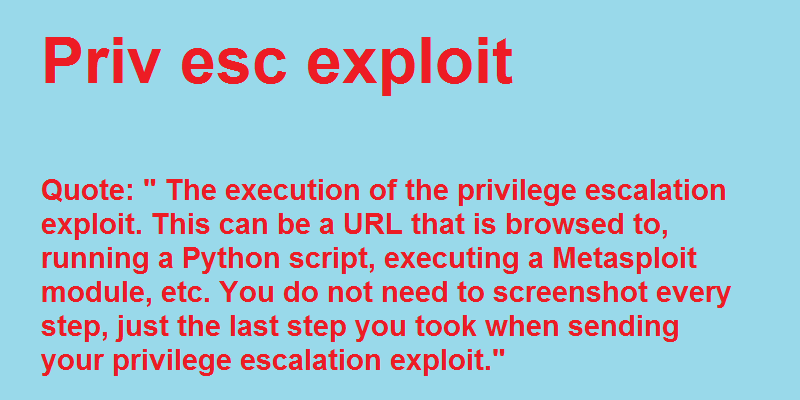
\includegraphics [width=\textwidth]{./hosts/\hostname/privescexploit.png}
%scale 0.5 bedeutet 50% der originalgröße
%angle=90 Grafik um 90° drehen
\caption[Priv escalation exploit of \hostname]{Priv escalation exploit of \hostname} \label{\hostname-3}
\end{figure}

\fi
%--------------------------------------End of Priv Esc Block------------------------

\subsubsection{Proof and Post escalation}
\begin{lstlisting}[caption={Post exploitation of \hostname},label=\hostname-post]
*@Post exploitation commands run:@*

\end{lstlisting}

\begin{figure}[H]
\centering
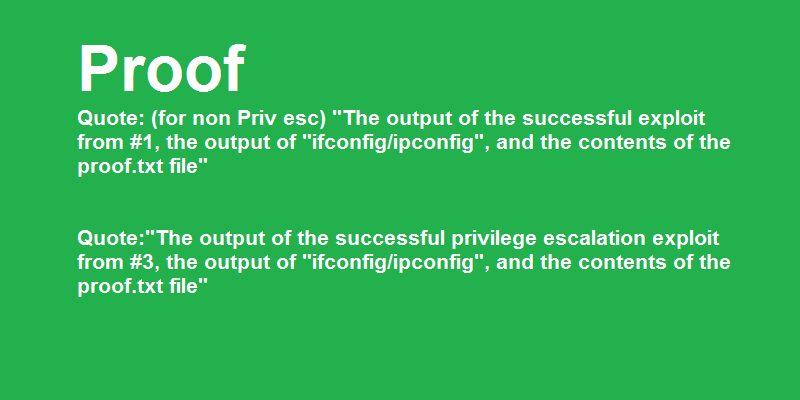
\includegraphics [width=\textwidth]{./hosts/\hostname/proof.png}
%scale 0.5 bedeutet 50% der originalgröße
%angle=90 Grafik um 90° drehen
\caption[Proof of \hostname]{Proof of \hostname} \label{\hostname-4}
\end{figure}


%---------------------End of host file
